\documentclass[11pt]{article}

\usepackage[doublespacing]{setspace}
% \usepackage[margin=1in]{geometry}

\usepackage{lipsum}
\usepackage{cite}
\usepackage{graphicx}


\title  {``Bees?''\\ A Large Scale, Co-operative Simulation 
         Weighing Altruism and Selfishness}
\author {Alexander Simms, Ravenna Thielstrom}
\date   {CS 81: Adaptive Robotics, Spring 2014}
\begin{document}
	\maketitle

	\begin{abstract}
		% A short abstract of 200 to 300 words summarizing your findings. 

		The Prisoner’s Dilemma, in philosophy, is a hypothetical situation that tests human nature. Two criminals are imprisoned and sentenced for 5 years. If, however, one prisoner should choose to betray the other, he will be set free and the betrayed prisoner will receive 10 years of prison. If, on the other hand, they simultaneously betray each other, both will receive the 10 year sentence. Silence from both parties gets them both the original, lesser punishment of 5 years. Although a human may argue that altruism is the best option for both parties, game theory states that in this situation, one should always choose to betray in order to minimize personal loss, and indeed one would expect this kind of decision from an artificial agent. Yet plenty of communities exist in nature that revolve around altruistic cooperation- for example, a bee colony, where individual bees retrieve nectar for the communal hive rather than scouting selfishly for their own survival. Although cooperation can certainly be implemented into an artificial life simulation, from an evolutionary standpoint a more interesting question is raised: can the interactions of a group and the parameters of their environment produce emergent cooperation among independent agents? This research aims to investigate the possibility of emergent altruism through evolutionary game theory. To this effect, we used NEAT to evolve neural-net topologies across many generations in a bee colony simulation, testing what possible circumstances might lead to altruistic decisions or selfish decisions in the hive. Initial speculation produced a hypothesis that the amount of altruism and selfishness demonstrated in NEAT-trained agents will be most affected by an individual fitness relying on group fitness. However, the results of our experiments demonstrate that while this is partly true and group fitness is key to altering artificial behavior, in the end selfishness wins out.

	\end{abstract}

	\section{Introduction} % (fold)
	\label{sec:introduction}
		% An introduction that contrasts your study with other related work. 
		% Find and read at least three articles related to your experiment and 
		% discuss these papers here. 
		\lipsum[3-8]
	% section introduction (end)

	\section{Experiments} % (fold)
	\label{sec:experiments}
		% A detailed description of your experiments. 
		% There should be enough information provided so that someone could 
		% reproduce your experiments. 

		\subsection{The Bee Model} % (fold)
		\label{sub:the_bee_model}
			To conduct these experiments, a model was developed that takes inspiration from the nectar-collecting hive insect, known in some circles as the bee. Our model consists of a population of individual neural nets, evolving by the NeuroEvolution of Adapting Topologies algorithm, henceforth referred to as NEAT.\cite{neat} NEAT, first developed by the illustrious Kenneth Stanley, is a genetic algorithm that has a flexible genetic encoding that allows for the topology of the network to grow and change over time, based on a user-defined measure of ``fitness''. All of the genes within the genetic encoding are tagged with historical markings, which allows for quick implementation of ``crossing-over,'' the process by which genetic information from an individual's parents is mixed. Finally, NEAT allows for speciation: individuals within the population are grouped together based on the similarness of their genomes, and only those individuals with similar genomes are allowed to reproduce. This allows for each species to find its own niche, and prevents any one species from outcompeting all of the others. It is because of these features that NEAT was selected for this task.

			Each individual NEAT agent within this model is called a ``bee'', and the population of all of the NEAT agents is called the ``hive''. Each ``day'' within this model, all of the bees leave the hive to go and find nectar. The nectar is represented in this model as a random floating-point number between 0 and 1. When it recieves this nectar, it has the choice to either be selfish or altruistic. If the bee decides to be selfish, it eats the nectar then and there. If it decides to be altruistic, it brings the nectar back to the hive, where all of the nectar brought back by altruistic bees is pooled and shared equally among all of the altruistic bees. The ``fitness'' in this system is simply how much nectar a bee was able to eat on a given day.
		% subsection the_bee_model (end)

		\subsection{Basic Experiment} % (fold)
		\label{sub:basic_experiment}
			An experiment was carried out to determine the workability of the model. In this experiment, each bee lived for only one day, and afterwards died. Their fitnesses determined the makeup of the next generation of bees: the most fit bees were bred to produce hopefully more fit offspring.

			\begin{figure}[tb]
				\begin{center}
					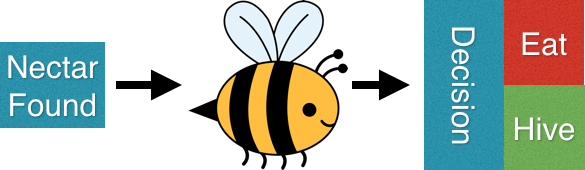
\includegraphics[scale=.5]{bee_diagrams/naive_system.png}
				\end{center}
				\caption{All that is fed into the system is the amount of nectar that the bee has found on that day, and the choice that the bee has made is determined by whether the output is closer to 0 or to 1.}
				\label{fig:naive_system}
			\end{figure}

			\begin{figure}[tb]
				\begin{center}
					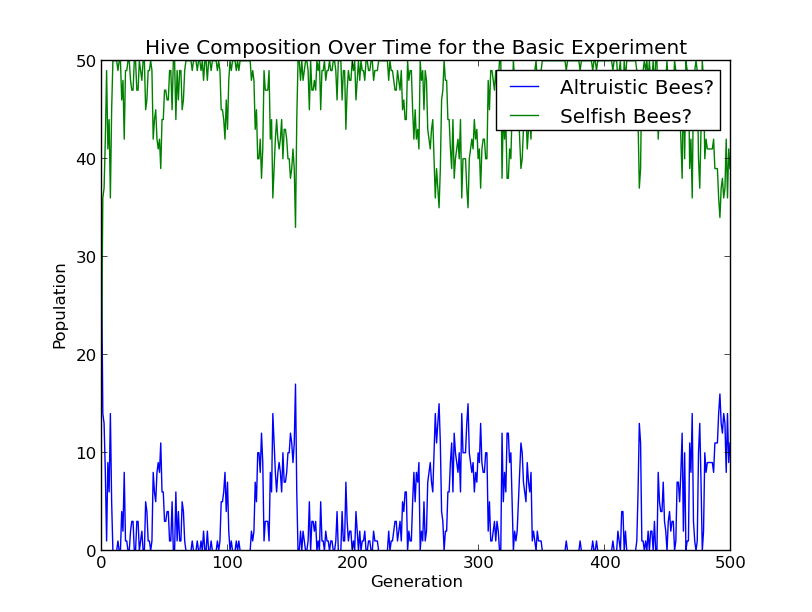
\includegraphics[scale=.75]{results/basic_comp.png}
				\end{center}
				\caption{Under the conditions of the basic experiment, altruism lost handily to selfishness.}
				\label{fig:figure1}
			\end{figure}
		% subsection basic_experiment (end)

		\subsection{Hive Fitness} % (fold)
		\label{sub:hive_fitness}
		\lipsum[10-12]
		% subsection hive_fitness (end)

		\subsection{Recurrent Networks} % (fold)
		\label{sub:recurrent_networks}
		\lipsum[12-14]
		% subsection recurrent_networks (end)

		\subsection{Advice from Bees} % (fold)
		\label{sub:advice_from_bees}
		
		% subsection advice_from_bees (end)

	% section experiments (end)

	\section{Discussion} % (fold)
	\label{sec:discussion}
	\lipsum[14-20]
	% section discussion (end)
	\singlespacing
	\appendix
	\pagebreak
	\section{NEAT Configurations} % (fold)
	\label{sec:neat_configurations}
	
		\subsection{Configuration for Basic Experiment} % (fold)
		\label{sub:configuration_for_basic_experiment}
			\begin{verbatim}
				[phenotype]
				input_nodes         = 1
				output_nodes        = 1
				max_weight          = 30
				min_weight          = -30
				feedforward         = 0
				nn_activation       = tanh 
				hidden_nodes        = 0
				weight_stdev        = 0.9

				[genetic]
				pop_size              = 50
				max_fitness_threshold = 1

				# Human reasoning
				prob_addconn          = 0.05
				prob_addnode          = 0.03
				prob_mutatebias       = 0.2
				bias_mutation_power   = 0.5
				prob_mutate_weight    = 0.9
				weight_mutation_power = 1.5
				prob_togglelink       = 0.01
				elitism               = 1

				[genotype compatibility]
				compatibility_threshold = 3.0
				compatibility_change    = 0.0
				excess_coeficient       = 1.0
				disjoint_coeficient     = 1.0
				weight_coeficient       = 0.4

				[species]
				species_size        = 10
				survival_threshold  = 0.2
				old_threshold       = 30
				youth_threshold     = 10
				old_penalty         = 0.2
				youth_boost         = 1.2
				max_stagnation      = 15
			\end{verbatim}
		% subsection configuration_for_basic_experiment (end)

		\pagebreak
		\subsection{Configuration for Hive Fitness} % (fold)
		\label{sub:configuration_for_hive_fitness}
			\begin{verbatim}
				[phenotype]
				input_nodes         = 1
				output_nodes        = 1
				max_weight          = 30
				min_weight          = -30
				feedforward         = 0
				nn_activation       = tanh 
				hidden_nodes        = 0
				weight_stdev        = 0.9

				[genetic]
				pop_size              = 50
				max_fitness_threshold = 1

				# Human reasoning
				prob_addconn          = 0.05
				prob_addnode          = 0.03
				prob_mutatebias       = 0.2
				bias_mutation_power   = 0.5
				prob_mutate_weight    = 0.9
				weight_mutation_power = 1.5
				prob_togglelink       = 0.01
				elitism               = 1

				[genotype compatibility]
				compatibility_threshold = 3.0
				compatibility_change    = 0.0
				excess_coeficient       = 1.0
				disjoint_coeficient     = 1.0
				weight_coeficient       = 0.4

				[species]
				species_size        = 10
				survival_threshold  = 0.2
				old_threshold       = 30
				youth_threshold     = 10
				old_penalty         = 0.2
				youth_boost         = 1.2
				max_stagnation      = 15
			\end{verbatim}
		% subsection configuration_for_hive_fitness (end)

		\pagebreak
		\subsection{Configuration for Recurrent Networks} % (fold)
		\label{sub:configuration_for_recurrent_networks}
			\begin{verbatim}
				[phenotype]
				input_nodes         = 4
				output_nodes        = 1
				max_weight          = 30
				min_weight          = -30
				feedforward         = 0
				nn_activation       = tanh 
				hidden_nodes        = 0
				weight_stdev        = 0.9

				[genetic]
				pop_size              = 50
				max_fitness_threshold = 1

				# Human reasoning
				prob_addconn          = 0.05
				prob_addnode          = 0.03
				prob_mutatebias       = 0.2
				bias_mutation_power   = 0.5
				prob_mutate_weight    = 0.9
				weight_mutation_power = 1.5
				prob_togglelink       = 0.01
				elitism               = 1

				[genotype compatibility]
				compatibility_threshold = 3.0
				compatibility_change    = 0.0
				excess_coeficient       = 1.0
				disjoint_coeficient     = 1.0
				weight_coeficient       = 0.4

				[species]
				species_size        = 10
				survival_threshold  = 0.2
				old_threshold       = 30
				youth_threshold     = 10
				old_penalty         = 0.2
				youth_boost         = 1.2
				max_stagnation      = 15
			\end{verbatim}
		% subsection configuration_for_recurrent_networks (end)
	% section neat_configurations (end)

	\nocite{*}
	\bibliography{bib}
	\bibliographystyle{plain}

\end{document}